\documentclass{../../text-style}

\texttitle{Лекция 9: Качество программного обеспечения}

\begin{document}

\maketitle
\thispagestyle{empty}

\attribution{Тимофей Александрович Брыксин, бывш. доцент кафедры системного программирования СПбГУ}

\section{Понятие качества ПО}

Основной проблемой в управлении качеством является тот факт, что популярное понимание качества слишком неясное и неоднозначное. 

\subsection{Популярный взгляд на качество}

Общепринятое мнение о качестве таково, что это нечто нематериальное и <<неосязаемое>>. Такие выражения как <<хорошее качество>> и <<плохое качество>> служат наглядным примером, как люди говорят о чем-нибудь неопределённом для них, то, что они не могут четко характеризовать и определить. Если попросить разных людей высказать свое мнение по поводу того, что такое качественное ПО, можно получить следующие варианты ответов:

\begin{itemize}
    \item его легко использовать;
    \item оно демонстрирует хорошую производительность;
    \item в нём нет ошибок;
    \item оно не портит пользовательские данные при сбоях;
    \item его можно использовать на разных платформах;
    \item оно может работать 24 часа в сутки и 7 дней в неделю;
    \item в него легко добавлять новые возможности;
    \item оно удовлетворяет потребности пользователей;
    \item оно хорошо документировано.
\end{itemize}

Такое мнение отражает тот факт, что люди воспринимают и интерпретируют качество по-разному. Подразумевается, что качество не может быть контролируемым и управляемым, и тем более оно не может быть количественно измеримым. Такой взгляд ярко контрастирует с профессиональным подходом к управлению качеством~--- качество это четко определенная величина, которую можно измерить и проконтролировать, она поддается управлению и улучшению.

\subsection{Профессиональный подход к качеству}

В 1979 году Philip B. Crosby определил качество как <<соответствие требованиям>> (``conformance to requirements''), а J.M. Juran и Frank M. Gryna в 1970 определили качество как <<пригодность к использованию>> (``fitness for use''). Эти два определения тесно связаны и прекрасно согласуются, как мы увидим чуть позже.

<<Соответствие требованиям>> предполагает, что требования должны быть настолько четко определены, что они не могут быть поняты и интерпретированы некорректно. Позже, на этапе разработки, производятся регулярные измерения разработанного продукта для определения соответствия требованиям. Любые несоответствия должны рассматриваться как дефекты~--- отсутствие качества. Например, спецификация на определенную модель радиостанции может требовать возможности принимать определенную частоту радиоволн на расстоянии более чем 30 километров от источника вещания. В случае, если радиостанция не способна выполнить данное требование, она не удовлетворяет требованию к качеству и должна быть признана негодной и некачественной.

Определение <<Пригодность к использованию>> принимает во внимание требования и ожидания конечных пользователей продукта, которые ожидают, что продукт или предоставляемый сервис будет удобным для их нужд. Однако разные пользователи могут использовать продукт по-разному, это означает, что продукт должен обладать максимально разнообразными вариантами использования. Согласно определению Juran и Gryna каждый вариант использования~--- это характеристика качества, и все они могут быть классифицированы по категориям в качестве параметров пригодности к использованию.

Эти два определения качества (<<соответствие требованиям>> и <<пригодность к использованию>>) по существу одинаковы. Разница в том, что вариант <<пригодность к использованию>> указывает на важную роль требований и ожиданий заказчика. Роль заказчика, связанная с качеством, никогда не может быть переоценена. С точки зрения заказчика, качество продукта, который он приобрел, состоит из множества различных факторов, таких как цена, производительность, надежность и т.д. Только ваш заказчик может рассказать вам о качестве, потому что это единственное, что он действительно покупает. Заказчик не покупает продукт. Он покупает ваши гарантии того, что все его ожидания к продукту будут реализованы.

Давайте еще раз попытаемся дать определение качеству с точки зрения заказчика или пользователя продукта. Качество~--- это пригодность к использованию: делает ли данный продукт то, в чем я нуждаюсь, облегчает ли он мою работу, могу ли я его использовать так, как мне удобно. А теперь посмотрим на точку зрения разработчика. Качество~--- это соответствие специфицированным и собранным требованиям: делает ли данный продукт все то, что указано в требованиях. Проблема в том, что специфицированные и собранные требования~--- это обычно лишь часть всех реальных требований и ожиданий заказчика. Где же правильное определение качества?

Качество~--- это соответствие реальным требованиям, явным и неявным. Очень часто неявные требования настолько очевидны для заказчика или пользователя, что он даже не предполагает, что они неизвестны разработчикам. И заказчик будет удовлетворен только тогда, когда купленный продукт будет полностью удовлетворять его реальным и жизненным требованиям, как специфицированным, так и нет.

Для того, чтобы как можно точнее определить и зафиксировать эти ожидания заказчика, в рамках работы с требованиями некоторые авторы выделяют даже отдельную дисциплину~--- управление требованиями к качеству (quality requirements management). Разработчики должны хорошо понимать смысл, вкладываемый в концепцию качества, характеристики и значение качества в отношении разрабатываемого или сопровождаемого программного обеспечения.

\subsection{Стоимость качества}

% https://asq.org/quality-resources/cost-of-quality

Движущей силой программных проектов является желание создать программное обеспечение, обладающее определенной ценностью. Ценность программного обеспечения может выражаться в денежной форме, а может и нет. Заказчик обычно имеет свое представление о максимальных стоимостных вложениях, возврат которых ожидается в случае достижения основных целей создания программного обеспечения. Но при этом заказчики часто не задумываются о вопросах качества и связанной с ними стоимостью. В таком случае крайне важно обеспечить высокую степень вовлечения заказчика в процесс принятия решений и полного понимания заказчиком стоимости и выгоды, связанной с достижением того или иного уровня качества. В идеальном случае большинство такого рода решений должно приниматься в процессе работы с требованиями, однако эти вопросы могут подниматься на протяжении всего жизненного цикла программного обеспечения. Не существует каких-то <<стандартных>> правил того, как именно необходимо принимать такие решения. Однако, инженеры должны быть способны представить различные альтернативы по достижению разных характеристик качества и их стоимость.

Стоимость качества может быть дифференцирована на:

\begin{itemize}
    \item стоимость предупреждения дефектов (prevention cost)~--- стоимость внедрения системы управления качеством для предупреждения дефектов,
    \item стоимость оценки (appraisal cost)~--- стоимость оценки того, насколько продукт соответствует требованиям по качеству,
    \item стоимость внутренних сбоев (internal failure cost)~--- стоимость, связанная с дефектами, выявленными до того, как продукт попал к пользователю,
    \item стоимость внешних сбоев (external failure cost)~--- стоимость, связанная с дефектами, выявленными после того, как продукт попал к пользователю.
\end{itemize}

\section{Модель качества ПО}

Качество продукта достигается процедурами контроля промежуточных продуктов на процессах ЖЦ, проверкой их на достижение необходимого качества, а также методами сопровождения продукта. Для эффективного отслеживания уровня качества вводят следующие три уровня представления.

Первый уровень соответствует определению характеристик (показателей) качества ПО, каждая из которых отражает отдельную точку зрения пользователя на качество. 

Второму уровню соответствуют атрибуты для каждой характеристики качества, которые детализируют разные аспекты конкретной характеристики. Набор атрибутов характеристик качества используется при оценке качества.

Третий уровень предназначен для измерения качества с помощью метрик, каждая из них определяется как комбинация метода измерения атрибута и шкалы измерения значений атрибутов. Также для каждой метрики часто вводят оценочный элемент метрики (вес), который используется для оценки количественного или качественного значения отдельного атрибута показателя ПО. В зависимости от назначения, особенностей и условий сопровождения ПО выбираются наиболее важные характеристики качества и их атрибуты. Выбранные атрибуты и их приоритеты часто отражаются в требованиях на разработку систем либо используются соответствующие приоритеты эталона класса ПО, к которому это ПО относится.

Существуют различные модели качества продукта, но мы будем придерживаться модели ISO/IEC 25010:2011. В ней выделяются следующие характеристики верхнего уровня:

\begin{itemize}
    \item функциональность;
    \item надежность;
    \item удобство использования;
    \item эффективность;
    \item сопровождаемость;
    \item переносимость.
\end{itemize}

Для каждой характеристики качества определяется набор атрибутов, влияющих на нее. В свою очередь для атрибутов определяются метрики. Метрики и позволяют измерять итоговое качество продукта. Рассмотрим характеристики по отдельности.

\begin{center}
    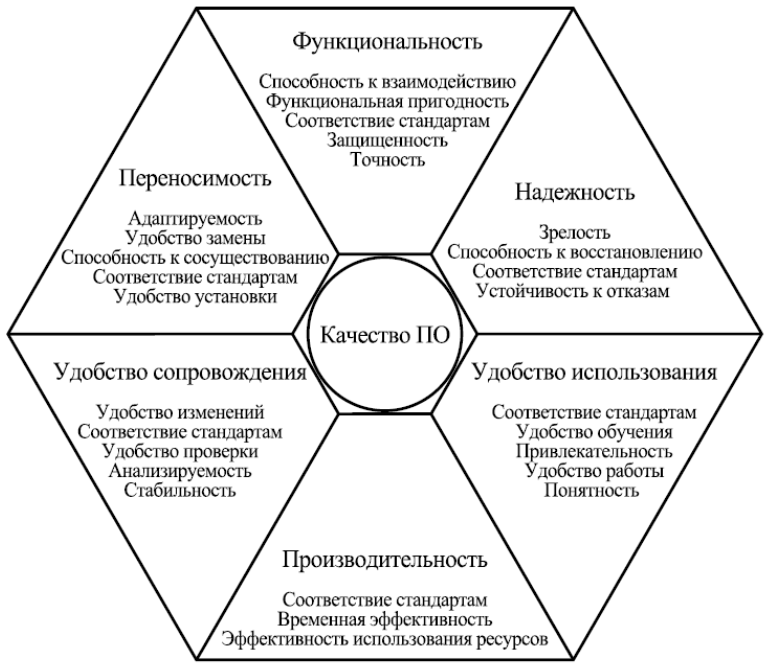
\includegraphics[width=0.7\textwidth]{qualityCharacteristics.png}
\end{center}

\subsection{Характеристики качества}

\paragraph{Функциональность}~--- совокупность свойств, определяющих способность ПО выполнять перечень функций в заданной среде и в соответствии с требованиями к обработке и общесистемным средствам. Под функцией понимается некоторая упорядоченная последовательность действий для удовлетворения потребительских свойств. Функции бывают целевые (основные) и вспомогательные.

К атрибутам функциональности относятся:

\begin{itemize}
    \item функциональная полнота (suitability)~--- свойство компонента, которое показывает степень достаточности основных функций для решения задач в соответствии с назначением ПО;
    \item правильность, точность (accuracy)~--- атрибут, который показывает степень достижения правильных результатов;
    \item способность к взаимодействию (interoperability)~--- это способность ПО работать с другими системами в процессе решения задачи (системные вызовы ОС, загрузка данных, проведение измерений с помощью внешних датчиков и т.д.);
    \item защищенность (security)~--- атрибут, который показывает способность ПО предотвращать несанкционированный доступ (случайный или умышленный) к программам и данным;
    \item соответствие стандартам и правилам (compliance)~--- соответствие ПО имеющимся индустриальным стандартам, нормативным и законодательным актам (что часто требуется при разработке финансового ПО, систем, работающих с личными данными пользователей).
\end{itemize}

Это качественные атрибуты, измерение которых может производиться с помощью довольно очевидных метрик. К примеру, пригодность определяется путем исполнения всех требуемых пользовательских сценариев с помощью созданного ПО.

\paragraph{Надежность}~--- совокупность атрибутов, которые определяют способность ПО преобразовывать исходные данные в результаты при условиях, зависящих от периода времени жизни. Снижение надежности ПО происходит из-за ошибок в требованиях, проектировании и выполнении.

К атрибутам надежности ПО относятся:

\begin{itemize}
    \item зрелость, завершенность, безотказность (maturity)~--- величина, обратная частоте отказов ПО. Обычно измеряется средним временем работы без сбоев. Чем менее часто ПО сбоит, тем более оно безотказно;
    \item устойчивость к отказам (fault tolerance)~--- способность ПО поддерживать заданный уровень работоспособности в заданных условиях. Такими условиями могут быть отказ сетевой инфраструктуры, нарушения в формате данных, нарушение работы окружения и т.д. Устойчивость к отказам~--- крайне важный атрибут, учитывать который нужно уже на стадии проектирования архитектуры ПО. В случае неустойчивого к отказам ПО компания может терять миллионы на постоянном восстановлении после отказов;
    \item способность к восстановлению (recoverability)~--- это способность ПО восстанавливать заданный уровень работоспособности после отказа. Как правило, в восстановление входит также восстановление целостности данных. Данный атрибут определяет не только требуемое время, но и дополнительные ресурсы (время персонала участвующего в восстановлении и т.д). Как правило, абсолютную устойчивость к отказам обеспечить невозможно. В таких случаях и становится важна способность к восстановление. Не можешь гарантировать, что не упадёт~--- гарантируй, что быстро поднимется.
\end{itemize}

К некоторым типам систем (реального времени, радарных, систем безопасности, коммуникации и др.) предъявляются требования для обеспечения высокой надежности (недопустимость ошибок, точность, достоверность, удобство применения и др.). Таким образом, надежность ПО в значительной степени зависит от числа оставшихся и не устраненных ошибок в процессе разработки на этапах ЖЦ. В ходе эксплуатации ошибки обнаруживаются и устраняются.

Если при исправлении ошибок не вносятся новые или, по крайней мере, новых ошибок вносится меньше, чем устраняется, то в ходе эксплуатации надежность ПО непрерывно возрастает. Чем интенсивнее проводится эксплуатация, тем интенсивнее выявляются ошибки и быстрее растет надежность ПО.

В инженерии надежности термин пригодноспособность (dependability) означает способность системы иметь свойства, желательные для пользователя, который уверен в качественном выполнении функций системы, заданных в требованиях. Данный термин определяется дополнительным количеством атрибутов, которыми должна обладать система, а именно:

\begin{itemize}
    \item готовность к использованию (availability);
    \item готовностью к непрерывному функционированию (reliability);
    \item безопасность для окружающей среды, т.е. способность системы не вызывать катастрофических последствий в случае отказа (safety);
    \item секретность и сохранность информации (сonfidentiality);
    \item способность к сохранению системы и устойчивости к самопроизвольному ее изменению (integrity);
    \item способность к эксплуатации ПО, простота выполнения операций обслуживания, а также устранения ошибок, восстановление системы после их устранения и т.п. (maintainability).
\end{itemize}

\paragraph{Удобство применения} характеризуется множеством атрибутов, которые показывают на необходимые и пригодные условия использования ПО заданным кругом пользователей для получения соответствующих результатов. Часто удобство применения определяется как специфическое множество атрибутов программного продукта, характеризующих его эргономичность.

К подхарактеристикам удобства применения относятся:

\begin{itemize}
    \item понимаемость (understandability)~--- показатель, обратный усилиям, затрачиваемым пользователями на восприятие основных концепций ПО и осознания последовательности их применения для решения конкретной бизнес-задачи. То есть это показатель усилий, которые требуется приложить пользователю для того, чтобы понять, как сделать конкретную задачу;
    \item изучаемость, легкость изучения (learnability)~--- атрибут, который определяет усилия пользователей на определение применимости ПО путем использования операционного контроля, диагностики, а также процедур, правил и документации;
    \item удобство работы (operability)~--- показатель, обратный усилиям, предпринимаемым пользователями для решения своих задач с помощью ПО. В отличие от понятности, здесь имеются в виду усилия, прилагаемые для работы с уже известной задачей, с уже известной последовательностью действий. Также можно выделить следующие податрибуты:
    \begin{itemize}
        \item оперативность показывает скорость отклика ПО на действия пользователя;
        \item согласованность~--- общая согласованность концепций работы с ПО с его окружением. Например, нехорошо, если все приложения на данной операционной системе используют встроенные уведомления, а вы используете свои собственные, да притом ещё и на другой стороне экрана;
    \end{itemize}
    \item привлекательность (attractiveness)~--- способность ПО быть привлекательным для пользователей. Сюда, например, можно включить модные плоские иконки или другие трендовые и ожидаемые элементы интерфейса.
\end{itemize}

\paragraph{Эффективность}~--- способность ПО при ограниченных ресурсах обеспечивать заданный уровень работоспособности. Иногда выделяют коэффициент~--- отношение ценности получаемых с помощью ПО результатов к затрачиваемым на это ресурсам.

К подхарактеристикам эффективности ПО относятся:

\begin{itemize}
    \item временная эффективность, реактивность (time behaviour)~--- способность ПО выдавать ожидаемые результаты за отведённое время. При этом измеряется не время отклика как таковое, а скорость работы в окружении (ответ на запросы от других сервисов, ответ на запросы от ОС и т.д.);
    \item эффективность ресурсов (resource utilisation)~--- атрибут, показывающий количество и продолжительность используемых ресурсов при выполнении функций ПО.
\end{itemize}

\paragraph{Сопровождаемость}~--- множество свойств, которые показывают на усилия, которые надо затратить на проведение модификаций, включающих корректировку, усовершенствование и адаптацию ПО при изменении среды, требований или функциональных спецификаций. В большинстве случаев данная характеристика важна для самих разработчиков, однако бывают и исключения (например, в случае аутсорсинга разработки без аутсорсинга сопровождения).

Cопровождаемость включает подхарактеристики:

\begin{itemize}
    \item анализируемость (analyzability)~--- атрибут, определяющий необходимые усилия для диагностики отказов или идентификации частей, которые будут модифицироваться;
    \item изменяемость (changeability)~--- атрибут, который определяет удаление ошибок в ПО или внесение изменений для их устранения, а также введение новых возможностей в ПО или в среду функционирования. Этот атрибут нужно учитывать еще на стадии проектирования архитектуры. Архитектура, позволяющая легко вносить изменения, сэкономит вам время и деньги как на стадии разработки, так и на стадии поддержки;
    \item стабильность (stability)~--- атрибут, указывающий на постоянство структуры и риск ее модификации. Это показатель, обратный риску возникновения неожиданных эффектов при внесении необходимых изменений;
    \item тестируемость (testability)~--- атрибут, показывающий на усилия при проведении валидации и верификации с целью обнаружения несоответствий требованиям, а также на необходимость проведения модификации ПО и сертификации.
\end{itemize}

\paragraph{Переносимость}~--- множество показателей, указывающих на способность ПО адаптироваться к работе в новых условиях среды выполнения. Среда может быть организационной, аппаратной и программной. Поэтому перенос ПО в новую среду выполнения может быть связан с совокупностью действий, направленных на обеспечение его функционирования в среде, отличной от той среды, в которой оно создавалось с учетом новых программных, организационных и технических возможностей.

Переносимость включает подхарактеристики:

\begin{itemize}
    \item адаптивность (adaptability)~--- атрибут, определяющий усилия, затрачиваемые на адаптацию к различным средам;
    \item настраиваемость, простота инсталляции (installability)~--- атрибут, который определяет необходимые усилия для запуска данного ПО в специальной среде;
    \item сосуществование (coexistence)~--- способность ПО сосуществовать с другими программами в общем окружении, разделяя с ними ресурсы и соблюдая правила работы в этом окружении;
    \item заменяемость (replaceability)~--- атрибут, который обеспечивает возможность интероперабельности при совместной работе с другими программами с необходимой инсталляцией или адаптацией ПО.
\end{itemize}

\subsection{Виды метрик}

% https://intuit.ru/studies/courses/2190/237/lecture/6136?page=3

Далее мы будем говорить о конкретных метриках. Полезно понимать, как эти метрики соответствуют описанным характеристикам:

\begin{itemize}
    \item Функциональность: метрики тестирования
    \item Надежность: метрики тестирования, динамические метрики
    \item Удобство использования: метрики эргономики
    \item Эффективность: динамические метрики
    \item Сопровождаемость: метрики кода
    \item Переносимость: метрики кода
\end{itemize}

Некоторые из метрик кода и тестирования мы рассмотрим подробнее далее.

В целом же обычно выделяют три типа метрик:

\begin{itemize}
    \item метрики программного продукта, которые используются при измерении его характеристик;
    \item метрики процесса, которые используются при измерении свойства процесса ЖЦ создания продукта;
    \item метрики использования, которые используются для измерения характеристик взаимодействия пользователя и продукта. К таким метрикам, в частности, относятся метрики эргономики, описывающие удобство продукта для конечного пользователя.
\end{itemize}

Метрики программного продукта включают:

\begin{itemize}
    \item внешние метрики, обозначающие свойства продукта, видимые пользователю:
    \begin{itemize}
        \item надежности продукта, которые служат для определения числа дефектов;
        \item функциональности, с помощью которых устанавливаются наличие и правильность реализации функций в продукте;
        \item сопровождения, с помощью которых измеряются ресурсы продукта (скорость, память, среда);
        \item применимости продукта, которые способствуют определению степени доступности для изучения и использования;
        \item стоимости, которыми определяется стоимость созданного продукта.
    \end{itemize}
    \item внутренние метрики, обозначающие свойства, видимые только команде разработчиков:
    \begin{itemize}
        \item метрики размера, необходимые для измерения продукта с помощью его внутренних характеристик;
        \item метрики сложности, необходимые для определения сложности продукта;
        \item метрики стиля, которые служат для определения подходов и технологий создания отдельных компонентов продукта и его документов.
    \end{itemize}
\end{itemize}

Внутренние метрики позволяют определить производительность продукта и являются релевантными по отношению к внешним метрикам.

Внешние и внутренние метрики задаются на этапе формирования требований к ПО и являются предметом планирования и управления достижением качества конечного программного продукта.

В качестве \emph{метрик процесса} могут быть время разработки, число ошибок, найденных на этапе тестирования и др. Практически используются следующие метрики процесса:

\begin{itemize}
    \item общее время разработки и отдельно время для каждой стадии;
    \item время модификации моделей;
    \item время выполнения работ на процессе;
    \item число найденных ошибок при инспектировании;
    \item стоимость проверки качества;
    \item стоимость процесса разработки;
    \item ...
\end{itemize}

Метрики использования служат для измерения степени удовлетворения потребностей пользователя при решении его задач. Они помогают оценить не свойства самой программы, а результаты ее эксплуатации~--- эксплуатационное качество. Примером может служить точность и полнота реализации задач пользователя, а также затраченные ресурсы (трудозатраты, производительность и др.) на эффективное решение задач пользователя. Оценка требований пользователя проводится с помощью внешних метрик.

\subsection{Объекты измерения}

Стандарт ISO/IEC 9126-2 определяет следующие типы мер:

\begin{itemize}
    \item мера размера ПО в разных единицах измерения (число функций, строк в программе, размер дисковой памяти и др.);
    \item мера времени (функционирования системы, выполнения компонента и др.);
    \item мера усилий (производительность труда, трудоемкость и др.);
    \item мера учета (количество ошибок, число отказов, ответов системы и др.).
\end{itemize}

Специальной мерой может служить уровень использования повторных компонентов и он измеряется как отношение размера продукта, изготовленного из готовых компонентов, к размеру системы в целом. Данная мера используется также при определении стоимости и качества ПО. Примеры метрик:

\begin{itemize}
    \item общее число объектов и число повторно используемых;
    \item общее число операций, повторно используемых и новых операций;
    \item число классов, наследующих специфические операции;
    \item число классов, от которых зависит данный класс;
    \item число пользователей класса или операций и др.
\end{itemize}

При оценке общего количества некоторых величин часто используются среднестатистические метрики (среднее число операций в классе, наследников класса или операций класса и др.). Как правило, меры в значительной степени являются субъективными и зависят от знаний экспертов, производящих количественные оценки атрибутов компонентов программного продукта.

Вообще метрик существует огромное количество, и вряд ли будет разумным высчитывать и отслеживать их все. Наиболее оправдан подход, когда в зависимости от вашей команды, принятого процесса или особенностей проекта вы выбираете наиболее критичные метрики, показывающие ваши слабые места, и пристально отслеживаете их. Когда вы понимаете, что какие-то проблемные места начинают выравниваться, вы можете немного ослабить внимание к ним и переключиться на что-то ещё. 

С примерами других метрик, не разбираемых в лекции, можно ознакомиться, например, по ссылке \url{https://www.ispras.ru/preprints/docs/prep_25_2013.pdf} (дата обращения: 16.04.2023).

\section{Метрики}

\subsection{Простейшие метрики}

Наиболее простой (хоть и сомнительной) метрикой является количество строк кода (LOC или KLOC в случае измерения в тысячах). Такая метрика дает некоторое представление об объеме проделанной работы, однако полагаться на неё нельзя. Размер кода может зависеть от очень разных параметров и далеко не всегда там, где больше кода~--- больше работы. Простейшим примером являются части кода, переписанные с объектно-ориентированного подхода на функциональный подход. Количество строк кода может уменьшиться значительно, а вот времени на написание этого кода требуется не меньше.

Также часто рассматривают метрику производительности (LOC/затраты). В принципе вместо LOC может использоваться другая метрика объема труда. В таком случае данная метрика может дать даже лучшее приближение. Аналогичное верно для удельной стоимости (затраты/LOC), для качества кода (число ошибок/LOC). Наконец, часто используется метрика документированности (число страниц документации/LOC).

Все эти метрики могут быть соответствующим образом изменены, чтобы давать лучшее приближение к реальным значениям в случае конкретного подхода разработки (например, документированность в случае ООП может быть выражена как (Число документированных методов) / (Общее число методов)).

Заметим, что иногда метрики удобно использовать не в качестве абсолютных показателей, а как показатели направления развития. В таком случае, даже самая приблизительная метрика даст понимание вектора развития той или иной части проекта.
Теперь рассмотрим более сложные метрики.

\subsection{Метрики Холстеда}

Метрики Холстеда~--- одни из самых первых метрик измерения сложности программ. В отличие от большинства таких метрик, метрики Холстеда являются количественным, а не качественными. То есть метрики не принимают в расчет специфику программ, их семантику, а работают с ними просто как с формальным языком. Строго говоря, метрики Холстеда позволяют определить сложность предложений некоторого формального языка. 

Используются следующие показатели:

\begin{itemize}
    \item Number of Unique Operators (NUOprtr)
    \item Number of Unique Operands (NUOprnd)
    \item Number of Operators (Noprtr)
    \item Number of Operands (Noprnd)
    \item Halstead Program Volume (HPVol) $= (Noprtr + Noprnd) \times log_2(NUOprtr + NUOprnd)$
    \item Halstead Difficulty (HDiff) $= (\frac{NUOprtr}{2}) \times (\frac{Noprnd}{NUOprnd})$
    \item Halstead Effort (HEff) $= HDiff \times HPVol$
\end{itemize}

Halstead Program Volume~--- это некоторый <<объем>> программы. Halstead Difficulty~--- это сложность единицы объема программы. Соответственно, сложность понимания всей программы есть Halstead Effort.

Считать эти метрики очень просто, однако в настоящий момент они довольно редко используются, поскольку являются слишком общими и никак не учитывают особенности используемой парадигмы программирования, подхода к разработке и т.п.

\subsection{Цикломатическая сложность}

Цикломатическая сложность~--- это уже качественная метрика. Она анализирует управляющий граф программы (как правило, конкретного метода) и на основе его пытается предположить итоговую сложность этого фрагмента кода. Такие метрики ещё называют метриками сложности потока управления программы.

Автоматическое измерение метрики легко реализуется, а её значения позволяют делать некоторые осмысленные выводы о сложности того или иного метода (по крайней мере, если у вас цикломатическая сложность 150, то программа совершенно точно слишком сложная).

Используется следующая формула:

$C = E - N + 2P$, где $E$~--- число ребер, $N$~--- число узлов, $P$~--- число компонент связности.

В общем случае значение этой метрики показывает число тестовых прогонов программы, для прохода всех ветвей графа потока управления.

Заметим, что данная формула не способна различать условные конструкции и циклы. Кроме того, цикломатическая сложность не обращает внимание на сложность предикатов условий. Для исправления этого недостатка создавались модификации метрики, такие как метрика Майерса и метрика Мак-Кейба-Хансена.

\subsection{Метрики С. Чидамбера и К. Кемерера}

Эти шесть метрик адаптированы для программ с объектно-ориентированным подходом. Они исследуют методы, деревья наследования, классы и т.д.

\subsubsection{WMC: Weighted Methods Per Class}
Допустим, что в классе $С$ определены $n$ методов со сложностью $C_1$, $C_2$, , ..., $C_n$. Для оценки сложности может быть выбрана любая метрика сложности (например, цикломатическая сложность). Главное~--- нормализовать эту метрику так, чтобы номинальная сложность для метода принимала значение 1. В этом случае

$$WMC = \sum_{i=1}^{n}C_i$$

Количество методов и их сложность являются индикатором затрат на реализацию и тестирование классов. Кроме того, чем больше методов, тем сложнее дерево наследования (все подклассы наследуют методы их родителей). С ростом количества методов в классе его применение становится все более специфическим, тем самым ограничивается возможность многократного использования. По этим причинам метрика WMC должна иметь разумно низкое значение.

Очень часто применяют упрощенную версию метрики. При этом полагают $C_i = 1$, и тогда WMC~--- количество методов в классе.

Возможны два противоположных варианта подсчёта методов в классе.

\begin{itemize}
    \item Подсчитываются только методы текущего класса. Унаследованные методы игнорируются. Обоснование~--- унаследованные методы уже подсчитаны в тех классах, где они определялись. Таким образом, инкрементность класса~--- лучший показатель его функциональных возможностей, который отражает его право на существование. Наиболее важным источником информации для понимания того, что делает класс, являются его собственные операции. Если класс не может отреагировать на сообщение (например, в нем отсутствует собственный метод), тогда он пошлет сообщение родителю.
    \item Подсчитываются методы, определенные в текущем классе, и все унаследованные методы. Этот подход подчеркивает важность пространства состояний в понимании класса (а не инкрементности класса).
\end{itemize}

Существует ряд промежуточных вариантов. Например, подсчитываются текущие методы и методы, прямо унаследованные от родителей. Аргумент в пользу данного подхода~--- на поведение дочернего класса наиболее сильно влияет специализация родительских классов.
На практике приемлем любой из описанных вариантов. Главное~--- не менять вариант учета от проекта к проекту. Только в этом случае обеспечивается корректный сбор метрических данных.

\subsubsection{DIT: Depth of Inheritance Tree}

DIT определяется как максимальная длина пути от листа до корня дерева наследования классов. Соответственно, для отдельного класса DIT, это длина максимального пути от данного класса до корневого класса в иерархии классов.

По мере роста DIT вероятно, что классы нижнего уровня будут наследовать много методов. Это приводит к трудностям в предсказании поведения класса. Высокая иерархия классов (большое значение DIT) приводит к большей сложности проекта, так как означает привлечение большего количества методов и классов.

Вместе с тем, большое значение DIT подразумевает, что многие методы могут использоваться многократно.

\subsubsection{NOC: Number of children}

Значение NOC равно количеству детей, то есть количеству непосредственных наследников класса в иерархии классов. С увеличением NOC возрастает многократность использования, так как наследование~--- это форма повторного использования. Однако при возрастании NOC ослабляется абстракция родительского класса. Это означает, что в действительности некоторые из детей уже не являются членами родительского класса и могут быть неправильно использованы. Кроме того, количество детей характеризует потенциальное влияние класса на проект. По мере роста NOC возрастает количество тестов, необходимых для проверки каждого ребенка.

Метрики DIT и NOC~--- количественные характеристики формы и размера структуры классов. Хорошо структурированная объектно-ориентированная система чаще бывает организована как лес классов, чем как сверхвысокое дерево. По мнению Г. Буча, следует строить сбалансированные по высоте и ширине структуры наследования: обычно не выше, чем 7 ± 2 уровня, и не шире, чем 7 ± 2 ветви. Однако, современная архитектурная мысль вообще отрицает наследование как средство переиспользования кода, и не рекомендует наследоваться от классов вовсе (только реализовывать интерфейсы).

\subsubsection{СВО: Coupling between object classes}

СВО~--- это количество сопряжений класса. Сопряжение образует вызов метода или свойства в другом классе.

Данная метрика характеризует статическую составляющую внешних связей классов. С ростом СВО многократность использования класса, вероятно, уменьшается. Очевидно, что чем больше независимость класса, тем легче его повторно использовать в другом приложении. Высокое значение СВО усложняет модификацию и тестирование, которое следует за выполнением модификации. Понятно, что, чем больше количество сопряжений, тем выше чувствительность всего проекта к изменениям в отдельных его частях. Минимизация межобъектных сопряжений улучшает модульность и содействует инкапсуляции проекта.
СВО для каждого класса должно иметь разумно низкое значение. Это согласуется с рекомендациями по уменьшению сопряжения стандартного программного обеспечения.

\subsubsection{RFC: Response For a Class}

Введем вспомогательное определение. Множество отклика класса RS~--- это множе­ство методов, которые могут выполняться в ответ на прибытие сообщений в объект этого класса. Формула для определения RS имеет вид:

$$RS = \{M\} \cup_{i} \{R_i\}$$

где $\{R_i\}$~--- множество методов, вызываемых методом $i$, $\{M\}$~--- множество всех методов в классе. Метрика RFC равна количеству методов во множестве отклика, то есть равна мощности этого множества $RS$.

Метрика RFC является мерой потенциального взаимодействия данного класса с другими классами, позволяет судить о динамике поведения соответствующего объекта в системе. Данная метрика характеризует динамическую составляющую внешних связей классов.

Если в ответ на сообщение может быть вызвано большое количество методов, то усложняется тестирование и отладка класса, так как от разработчика тестов требуется больший уровень понимания класса, растет длина тестовой последова­тельности.

С ростом RFC увеличивается сложность класса. Наихудшая величина отклика может использоваться при определении времени тестирования.

\subsubsection{LCOM: Lack of Cohesion in Methods}

Каждый метод внутри класса обращается к одному или нескольким атрибутам (экземплярным переменным). Метрика LCOM показывает, насколько методы не связаны друг с другом через атрибуты (переменные). Если все методы обращаются к одинаковым атрибутам, то LCOM = 0.

Введем обозначения:

\begin{itemize}
    \item NotRelated~--- количество пар методов без общих экземплярных переменных;
    \item Related~--- количество пар методов с общими экземплярными переменными;
    \item $I_j$~--- набор экземплярных переменных, используемых методом $М_j$.
\end{itemize}

Очевидно, что

$$NotRelated = card\{I_{ij}\ |\ I_i \cap I_j = \emptyset\}$$
$$Related = card\{I_{ij}\ |\ I_i \cap I_j \neq \emptyset\}$$

Тогда  формула для вычисления недостатка связности в методах примет вид:

\begin{equation}
    LCOM=\begin{cases}
        NotRelated - Related, & \text{если}\ NotRelated > Related.\\
        0,                    & \text{в противном случае}.
    \end{cases}
\end{equation}

Можно определить метрику по-другому: LCOM~--- это количество пар методов, не связанных по атрибутам класса, минус количество пар методов, имеющих такую связь.

Недостаток связанности, то есть значение больше нуля, является свидетельством того, что класс следует разделить на два или более меньших подклассов.

Связность методов внутри класса должна быть высокой, так как это содействует инкапсуляции. Если LCOM имеет высокое значение, то методы слабо связаны друг с другом через атрибуты. Это увеличивает сложность, в связи с чем возрастает вероятность ошибок при проектировании. Высокие значения LСОМ означают, что класс, вероятно, надо спроектировать лучше (разбиением на два или более отдельных класса). Любое вычисление LCOM помогает определить недостатки в проектировании классов, так как эта метрика характеризует качество упаковки данных и методов в оболочку класса.

Вывод: связность в классе желательно сохранять высокой, то есть следует до­биваться низкого значения LCOM. 

Набор метрик Чидамбера-Кемерера~--- одна из пионерских работ по комплексной оценке качества объектно-ориентированного проектирования. Известны многочисленные предложения по усовершенствованию, развитию данного набора. Рассмотрим некоторые из них.

Недостатком метрики WMC является зависимость от реализации. Рассмотрим класс, предлагающий операцию интегрирования. Возможны две реализации:

\begin{enumerate}
    \item несколько простых операций:
    \begin{minted}{c}
SetInterval(min, max),
SetMethod(method),
SetPrecision(precision),
SetFunctionToIntegrate(function),
Integrate();
    \end{minted}
    \item одна сложная операция:
    \begin{minted}{c}
Integrate(function, min, max, method, precision);
    \end{minted}
\end{enumerate}

Для обеспечения независимости от этих реализаций можно предложить метрику WMC2:

$$WMC2 = \sum_{i=1}^{n}\text{количество параметров i-го метода}$$

Для нашего примера WMC2 = 5 и для первой и для второй реализации. Заметим, для первой реализации WMC = 5, а для второй реализации WMC = 1.

Дополнительно можно определить метрику Среднее число аргументов метода ANAM (Average Number of Arguments per Method): $ANAM = \frac{WMC2}{WMC}$.

Полезность метрики ANAM объяснить еще легче. Она ориентирована на принятые в объектно-ориентированном проектировании решения~--- применять простые операции с малым количеством аргументов, а не сложные операции с многочисленными аргументами.

Самые большие нарекания вызвала метрика LCOM: исследователи выявили несколько аномалий ее поведения:

\begin{itemize}
    \item LCOM дает нулевое значение для классов с самой разной связностью (см. пример ниже: класс B очевидно стоит разделить на два, но для него значение метрики равно 0). Для преодоления этой проблемы была предложена метрика $LCOM^*$.
    \item LСОМ учитывает связность методов только по данным, оставляя без внимания остальные механизмы их взаимодействия. Как следствие, классы с самой разной связностью имеют одинаковое значение LCOM.
    \item LCOM не рассматривает возможность доступа к данным класса через атрибуты с помощью функций get()/set(). Для таких классов может ошибочно формиро­ваться высокое значение метрики.
\end{itemize}

\begin{center}
    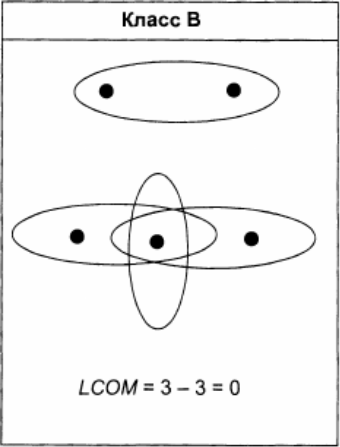
\includegraphics[width=0.3\textwidth]{lcomFail.png}
\end{center}

Б. Хендерсон-Селлерс, Л. Константайн и И. Грэхем предложили дополнитель­ную метрику $LCOM^*$. Нулевое значение метрики свидетельствует о высокой, хорошей связности, а высокое~--- о плохой связности. Формула для $LCOM^*$ имеет вид:

$$LCOM^* = \frac{(\frac{1}{a}\sum_{j=1}^{a}m(A_j)) - m}{1 - m}$$

где $m$~--- количество методов класса, $a$~--- количество атрибутов класса, $m(A_j)$~--- количество методов, которые имеют доступ к атрибуту $A$.

Если каждый метод имеет доступ ко всем атрибутам, значение метрики равно нулю (максимально хорошая связность). Если каждый метод работает только с од­ним, <<своим>> атрибутом, метрика дает единичное значение (максимально плохая связность). При наличии атрибутов, которые недоступны методам класса, значение метрики изменяется в диапазоне от 1 до 2. Такие значения свидетельствуют об ошибке проектирования (например, в классе есть <<мёртвые>> атрибуты или атрибуты, доступные только из внешней среды). Наконец, при нулевом количестве атрибутов или единственном методе метрика $LCOM^*$ не определена.

\subsection{Метрики Лоренца и Кидда}

\paragraph{Метрики, ориентированные на классы.} М. Лоренц и Д. Кидд подразделяют метрики, ориентированные на классы, на четыре категории: метрики размера, метрики наследования, внутренние и внешние метрики. Размерно-ориентированные метрики основаны на подсчете атрибутов и опера­ций для отдельных классов, а также их средних значений для всей ОО-системы. Метрики наследования акцентируют внимание на способе повторного использования операций в иерархии классов. Внутренние метрики классов рассматривают вопросы связности и кодирования. Внешние метрики исследуют сопряжение и повторное использование.

\paragraph{Размер класса, CS (Class Size)} Общий размер класса определяется с помощью следующих измерений:

\begin{itemize}
    \item общее количество операций (вместе с приватными и наследуемыми экземплярными операциями), которые инкапсулируются внутри класса;
    \item количество атрибутов (вместе с приватными и наследуемыми экземплярными атрибутами), которые инкапсулируются классом.
\end{itemize}

Метрика WMC Чидамбера и Кемерера также является взвешенной метрикой размера класса.

Большие значения CS указывают, что класс имеет слишком много обязанностей. Они уменьшают возможность повторного использования класса, усложняют его реализацию и тестирование.

При определении размера класса унаследованным (публичным) операциям и атрибутам придают больший удельный вес. Причина~--- приватные операции и атрибуты обеспечивают специализацию и более локализованы в проекте.

Могут вычисляться также средние количества атрибутов и операций класса. Чем меньше среднее значение размера, тем больше вероятность повторного использования класса. 
Рекомендуемое значение CS < 20 методов.

\paragraph{Количество операций, переопределяемых подклассом, NOO (Number of Operations Overridden by a Subclass).} Большие значения NOO обычно указывают на проблемы проектирования. Ясно, что подкласс должен расширять операции суперкласса. Если NOO велико, то разработчик с большой вероятностью нарушает абстракцию суперкласса: в какой-то момент вы просто не сможете гарантировать, что принцип подстановки Лисков до сих пор выполняется.  Это ослабляет иерархию классов, усложняет тестирование и модификацию программного обеспечения.
Рекомендуемое значение NOO <= 3 методов.

\paragraph{Количество операций, добавленных подклассом, NOA (Number of Operations Added by a Subclass).} Подклассы специализируются добавлением приватных операций и атрибутов. С ро­стом NOA подкласс удаляется от абстракции суперкласса. Обычно при увеличении высоты иерархии классов (увеличении DIT) должно уменьшаться значение NOA на нижних уровнях иерархии.

Для рекомендуемых значений CS = 20 и DIT = 6 рекомендуемое значение NOA <= 4 методов (для класса-листа).

\paragraph{Индекс специализации, SI (Specialization Index).} Обеспечивает грубую оценку степени специализации каждого подкласса. Специали­зация достигается добавлением, удалением или переопределением операций.

$$SI = (NOO \times \text{уровень}) / M_\text{общ.}$$

где уровень~--- номер уровня в иерархии, на котором находится подкласс, $M_{\text{общ}}$~--- общее количество методов класса.

Чем выше значение SI, тем больше вероятность того, что в иерархии классов есть классы, нарушающие абстракцию суперкласса.

Рекомендуемое значение SI <= 0,15.

Пример расчета индексов специализации приведен ниже:

\begin{center}
    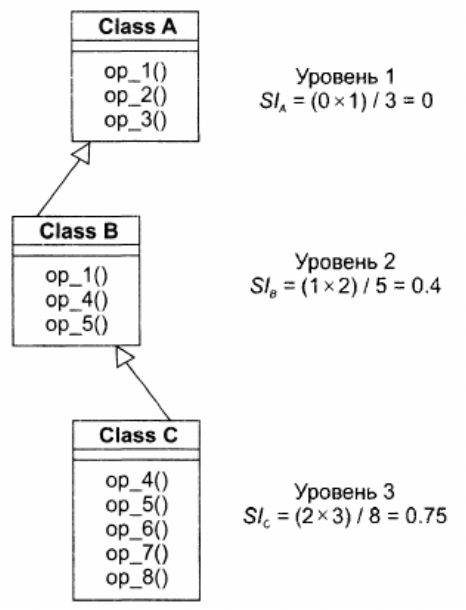
\includegraphics[width=0.4\textwidth]{siCalculation.png}
\end{center}

\paragraph{Метрики, ориентированные на операции.} Эта группа метрик ориентирована на оценку операций в классах. Обычно методы имеют тенденцию быть небольшими как по размеру, так и по логической сложности. Тем не менее реальные характеристики операций могут быть полезны для глубокого понимания системы.

\paragraph{Средний размер операции, $OS_{avg}$ (Average Operation Size).} В качестве индикатора размера может использоваться количество строк программы, однако LOC-оценки приводят к известным проблемам. Альтернативный вариант~--- <<количество сообщений, посланных операцией>>.

Рост значения метрики означает, что обязанности размещены в классе не очень удачно. Рекомендуемое значение $OS_{avg}$ <= 9.

\paragraph{Сложность операции, ОС (Operation Complexity).} Сложность операции может вычисляться с помощью стандартных метрик сложности, то есть с помощью LOC-оценок, метрики цикломатической сложности, метрики Холстеда или чего-то ещё. Поскольку операция должна быть ограничена конкретной обязанностью, желательно уменьшать ОС.

\paragraph{Среднее количество параметров на операцию, $NP_{avg}$ (Average Number of Parameters per operation).} Чем больше параметров у операции, тем сложнее сотрудничество между объектами. Поэтому значение $NP_{avg}$ должно быть как можно меньшим. Рекомендуемое значение $NP_{avg}$ <= 0,7.

Метрики Лоренца и Кидда~--- это скорее практические метрики, чем академические. Для них легко написать утилиты автоматического анализа кода, а сами метрики дают вполне осмысленную информацию о сложности кода.

\subsection{Набор метрик Фернандо Абреу}

Это довольно известный набор метрик объектно-ориентированного кода. Основными целями MOOD\footnote{Metrics for Object-Oriented Design}-метрик являются:

\begin{itemize}
    \item покрытие базовых механизмов объектно-ориентированной парадигмы, таких как инкапсуляция, наследование, полиморфизм, посылка сообщений;
    \item формальное определение метрик, позволяющее избежать субъективного измерения;
    \item независимость от размера оцениваемого программного продукта;
    \item независимость от языка программирования, на котором написан оцениваемый продукт.
\end{itemize}

Рассмотрим каждую из метрик по отдельности.

\paragraph{Фактор закрытости метода MHF (Method Hiding Factor).} Данная метрика определяет, насколько закрыты методы классов, то есть каково отношение интерфейсных методов, доступных клиентскому коду, у классов к общему числу методов.

Данную метрику следует интерпретировать исключительно в связи с кодом анализируемого проекта. Для разных проектов разные значения метрики могут быть приемлемы.

Используется следующая формула:

$$MHF = \frac{\sum\limits_{i=1}^{TC}M_h(C_i)}{\sum\limits_{i=1}^{TC}M_d(C_i)}$$

где $M_h(C_i)$~--- количество private-методов в классе $C_i$, $M_d(C_i)$~--- общее количество методов в классе $C_i$ (без унаследованных).

С увеличением MHF уменьшаются плотность дефектов в системе и затраты на их устранение. Обычно разработка класса представляет собой пошаговый процесс, при котором к классу добавляется все больше и больше деталей (скрытых методов). Такая схема разработки способствует возрастанию как значения МНF, так и качества класса.

\paragraph{Фактор закрытости свойства AHF (Attribute Hiding Factor).} Данная метрика определяет, насколько закрыты атрибуты классов, то есть каково отношение открытых атрибутов классов к общему числу атрибутов.

Нужно отметить, что в абсолютном большинстве случаев рекомендуется закрывать все атрибуты. Соответственно, данная метрика за редким исключением должна быть равна 1.

Используется следующая формула:

$$AHF = \frac{\sum\limits_{i=1}^{TC}A_h(C_i)}{\sum\limits_{i=1}^{TC}A_d(C_i)}$$

где $A_h(C_i)$~--- количество private-атрибутов в классе $C_i$, $A_d(C_i)$~--- общее количество атрибутов в классе $C_i$.

В идеальном случае все атрибуты должны быть скрыты и доступны только для методов соответствующего класса (AHF = 1).

\paragraph{Фактор наследования метода MIF (Method Inheritance Factor).} Данная метрика показывает, насколько часто используется наследование методов без переопределения, то есть каково отношение унаследованных и не переопределенных методов к общему числу методов.

Используется следующая формула:

$$MIF = \frac{\sum\limits_{i=1}^{TC}M_i(C_i)}{\sum\limits_{i=1}^{TC}M_a(C_i)}$$

где $M_i(C_i)$~--- количество унаследованных и не переопределенных методов в классе $C_i$, $M_a(C_i)$~--- общее количество методов в классе $C_i$.

Значение MIF, равное 0, указывает, что в системе отсутствует эффективное наследование, например, все унаследованные методы переопределены.

\paragraph{Фактор наследования свойства AIF (Attribute Inheritance Factor).} Данная метрика показывает, насколько часто используется наследование атрибутов без переопределения, то есть каково отношение унаследованных и не переопределенных атрибутов к общему числу атрибутов.

Используется следующая формула:

$$AIF = \frac{\sum\limits_{i=1}^{TC}A_i(C_i)}{\sum\limits_{i=1}^{TC}A_a(C_i)}$$

где $A_i(C_i)$~--- количество унаследованных и не переопределенных атрибутов в классе $C_i$, $A_a(C_i)$~--- общее количество атрибутов в классе $C_i$.

\paragraph{Фактор полиморфизма POF (Polymorphism Factor).} 
Данная метрика показывает, насколько часто используется полиморфизм в программе.

Используется следующая формула:

$$POF = \frac{\sum\limits_{i=1}^{TC}M_o(C_i)}{\sum\limits_{i=1}^{TC}M_n(C_i) \times DC(C_i)}$$

где $M_o(C_i)$~--- количество унаследованных и переопределенных методов в $C_i$, s, $DC(C_i)$~--- количество потомков класса $C_i$.

Числитель POF фиксирует реальное количество возможных полиморфных ситуаций. Очевидно, что сообщение, посланное в класс $C_i$, связывается (статически или динамически) с реализацией именуемого метода. Этот метод, в свою очередь, может или представляться несколькими <<формами>>, или переопределяться (в потомках $C_i$).

Знаменатель POF представляет максимальное количество возможных полиморфных ситуаций для класса $C_i$. Имеется в виду случай, когда все новые методы, определенные в $C_i$, переопределяются во всех его потомках.

Таким образом отношение показывает степень полиморфности созданного кода. Конечно, полиморфизм это хорошо, однако не стоит возводить его в абсолют. Помните, что полиморфный код сложнее понимать и сложнее изменять.

\paragraph{Фактор сопряжения COF (Coupling Factor).} Данный фактор показывает общее сопряжение построенной иерархии. Сопряжение фиксирует наличие между классами отношений клиент-поставшик (client-supplier). Отношение клиент-поставщик ($С_c$ => $С_s$) здесь означает, что класс-клиент содержит по меньшей мере одну не унаследованную ссылку на атрибут или метод класса-поставщика.

Используется следующая формула:

$$COF = \frac{\sum\limits_{i=1}^{TC}\Biggl(\sum\limits_{j=1}^{TC}is\_client(C_i, C_j)\Biggl)}{TC^2 - TC}$$

\begin{equation*}
    is\_client(C_c, C_s) = \begin{cases}
        1, & \text{если}\ C_c => C_s \cap C_c \neq C_s \\
        0, & \text{в противном случае}.
    \end{cases}
\end{equation*}

Знаменатель COF соответствует максимально возможному количеству сопряжений в системе с TC классами (потенциально каждый класс может быть поставщиком для других классов). Из рассмотрения исключены рефлексивные отношения, когда класс является собственным поставщиком. Числитель COF фиксирует реальное количество сопряжений.

С увеличением сопряжения классов плотности дефектов и затрат на доработку также возрастают. Сопряжения отрицательно влияют на качество ПО, их нужно сводить к минимуму. Практическое применение этой метрики доказывает, что сопряжение увеличивает сложность, уменьшает инкапсуляцию и возможности повторного использования, затрудняет понимание и сопровождаемость ПО.

Это довольно важная метрика, показывающая реальное качество построенной архитектуры.

\subsection{Метрики для объектно-ориентированного тестирования}

Кроме обычных метрик кода используются и специальные метрики тестирования. Эти метрики измеряют пригодность кода для тестирования. В частности, особое внимание уделяется следующим характеристикам кода.

\begin{itemize}
    \item Недостаток связности в методах.
    \item Процент публичных и защищенных методов: чем больше данный процент, тем проще тестировать классы.
    \item Публичный доступ к атрибутам: делать атрибуты публичными для тестирования~--- плохая практика.
    \item Количество корневых классов: чем больше корневых классов, тем больше кардинально различных паттернов поведения тестировать.
    \item Количество детей, высота дерева наследования: чем сложнее дерево наследования, тем сложнее тестировать поведение.
    \item Процентное количество не переопределенных запросов. 
    \item Процентное количество полиморфных вызовов: чем их больше, тем сложнее понимать код, тем сложнее тестировать.
    \item Скачок класса, системы: это процесс передачи управления между разными иерархиями классов, разными модулями системы. Такое поведение очень сложно качественно протестировать.
\end{itemize}

\section{Аудит программного кода}

Метрики являются исходными данными для проведения так называемого аудита программного кода. В процесса такого аудита проводится анализ программного кода, измеряются его характеристики и определяются проблемные места. Аудит может проводиться как экспертом, так и автоматически.

В случае экспертного аудита~--- это целый процесс, в рамках которого эксперт производит анализ кода, общается с командой и т.д. По результатам эксперт составляет отчет, основываясь на котором команда перерабатывает код проекта. Таким образом привлечение эксперта это исключительная ситуация, которая может изменить вектор развития проекта и существенно изменить характеристики его качества.

В случае автоматического аудита он может производиться при каждом изменении кода. При таком аудите проводится измерение основных характеристик с помощью заранее определенных метрик. Примером таких автоматических инструментов является \url{https://www.codacy.com/}. Автоматический аудит используется для непрерывного поддержания качества продукта.

Также может производиться постоянный расчет метрик ручным трудом кого-то из команды, однако это крайне сомнительная затея. Как правило, производить такой расчет после каждого изменения кода команде быстро надоест и процесс перестанет быть непрерывным.

\end{document}